 \section{Data Types}
\label{sec:data_types}

The \sunpypkg package provides two core data types that are designed to provide a general, standard, and consistent interface for loading and representing solar data across instruments and missions.
The core data types currently provided in \sunpypkg are \Timeseries and \Map, which support 1D temporal data and 2D image data, respectively. 
The purpose of these core classes is to accommodate the user with a standard data structure regardless of the data source (e.g. observational data from separate instruments). 
They maintain a consistent interface for accessing solar data attributes such as the data array itself as well as the meta data and relevant units, allowing for an easier workflow in the analysis of solar data observations.
They also include functionality for data manipulation and data visualization. 
This section provides an overview of the \Timeseries and \Map data types.

\subsection{\Timeseries}
\label{sec:timeseries}
Many observations in the field of solar physics consists of time series data. 
For example, the X-ray Sensor aboard the Geostationary Operational Environmental Satellite (GOES), which is used as the classification standard for solar flares, continuously measures the solar integrated X-ray flux as a function of time in two broadband channels. 
The \Timeseries class in \sunpypkg aims to accommodate the necessary requirements to represent solar time series data by providing a single, consistent interface for users to interact with and manipulate time series data from a variety of instruments. 

Users can add, truncate, re-sample, and combine data within a single \Timeseries or combine multiple \Timeseries together. 
Similar to \Map (Section \ref{sec:map}), \Timeseries has its own visualization methods to allow for easy inspection of the data.
An example of the GOES X-ray sensor \Timeseries  is shown in Figure~\ref{fig:timeseries_example}.

\begin{figure}
    \centering
    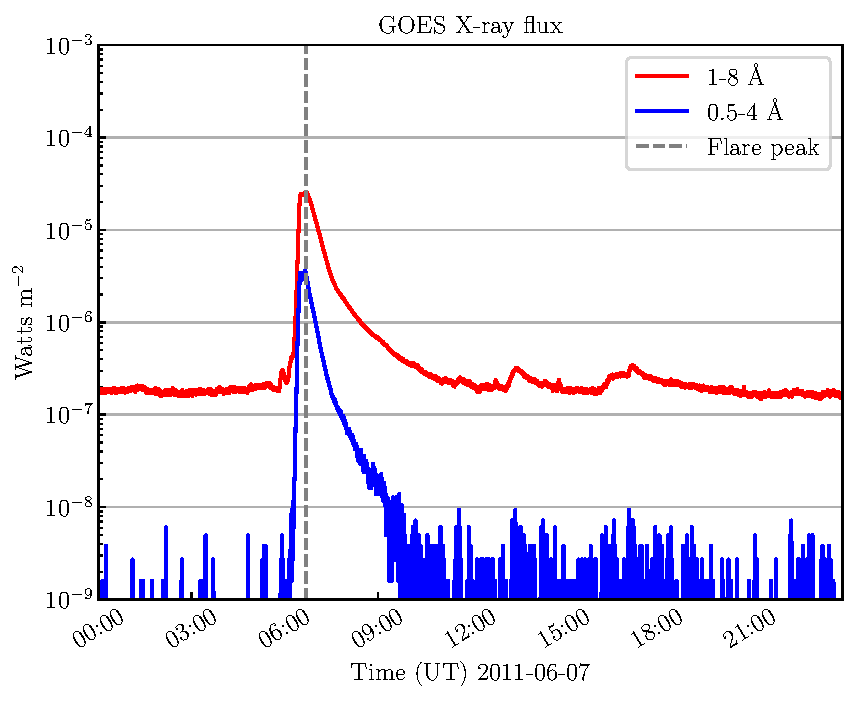
\includegraphics[width=0.55\textwidth]{figures/timeseries_example.pdf}
    \caption{An example of a GOES X-ray Sensor \Timeseries plotting the two broadband channels 1--8~\AA\ and 0.5--4~\AA\ over a 24 hour period. A solar flare is noted by the increase in flux and the grey dashed line denotes the flare peak as found from the Helio Event Knowledgebase (HEK).}
    \label{fig:timeseries_example}
\end{figure}

\Timeseries currently supports the data sources listed in Table \ref{tab:instruments} in addition to indices from the National Oceanic and Atmospheric (NOAA) Space Weather Prediction Center (SWPC) that track the solar cycle and its predicted progression. Due to its flexible data structure, it is easy to add additional instruments and data sources to the \Timeseries object.

%%%%%%%%%%%%%%%% TABLE %%%%%%%%%%%%%%%%%%%
\begin{table}
\begin{center}
\begin{tabular}{|p{12cm}|c|c|}
\hline
& \\
\textbf{Supported by \Timeseries}& \textbf{Instrument reference}\\
\hline
\hline
\textit{Geostationary Operational Environmental Satellite (GOES)} X-ray Sensor (XRS) & \citep{garcia94, hanser96} \\
\hline
\textit{Fermi} Gamma-ray Burst Monitor (GBM) &  \citep{meegan2009fermi} \\
\hline
\textit{Nobeyama Radioheliograph (NoRH)} & \citep{nakajima1994nobeyama} \\
\hline
\textit{PRoject for Onboard Autonomy (PROBA2)} Large Yield Radiometer (LYRA) & \citep{dominique2013lyra} \\
\hline
\textit{Solar Dynamics Observatory (SDO)} EUV Variability Experiment (EVE) & \citep{woods2010extreme}  \\
\hline
\textit{Reuven Ramaty High Energy Solar Spectroscopic Imager (RHESSI)} & \citep{lin2003reuven} \\
\hline
 & \\
\textbf{Supported by \Map} & \textbf{Instrument reference} \\
\hline
\hline
\textit{COronal Solar Magnetism Observatory (COSMO)} K-coronagraph (K-Cor) & \citep{dewijn12} \\
\hline
\textit{Hinode} X-Ray Telescope (XRT) & \citep{golub2008x}  \\
\hline
\textit{Interface Region Imaging Spectrograph (IRIS)} Slit Jaw Imager (SJI) & \citep{DePontieu2014}  \\
\hline
\textit{PRoject for Onboard Autonomy (PROBA2)} Sun Watcher using Active Pixel System detector and Image Processing (SWAP) & \citep{seaton2013swap} \\
\hline
\textit{Reuven Ramaty High Energy Solar Spectroscopic Imager (RHESSI)} & \citep{lin2003reuven} \\
\hline
\textit{Solar and Heliospheric Observatory (SOHO)} Extreme ultraviolet Imaging Telescope (EIT) & \citep{delaboudiniere1995eit}\\
\hline
\textit{Solar and Heliospheric Observatory (SOHO)} Large Angle Spectroscopic COronagraph (LASCO) & \citep{brueckner1995large} \\
\hline
\textit{Solar and Heliospheric Observatory (SOHO)} Michelson Doppler Imager (MDI) & \citep{scherrer1995solar}\\
\hline
\textit{Solar Dynamics Observatory (SDO)} Atmospheric Imaging Assembly (AIA) & \citep{lemen2012} \\
\hline
\textit{Solar Dynamics Observatory (SDO)} Helioseismic and Magnetic Imager (HMI) & \citep{schou12}  \\
\hline
\textit{Solar TErrestrial RElations Observatory (STEREO)} Extreme Ultraviolet Imager (EUVI), COronagraph 1 and 2 (COR1/2) for both \textit{STEREO} A and B & \citep{howard2008sun} \\
\hline
\textit{Transition Region and Coronal Explorer (TRACE)}  & \citep{handy99}  \\
\hline
\textit{Yohkoh} Soft X-ray Telescope (SXT) & \citep{tsuneta1991soft}  \\
\hline
\end{tabular}
\end{center}
\caption{The following table outlines the instruments supported by the \Timeseries and \Map objects described in Section \ref{sec:data_types}.}
\label{tab:instruments}
\end{table}
%%%%%%%%%%%%%%%% TABLE %%%%%%%%%%%%%%%%%%%

\subsection{\Map}
\label{sec:map}
Many types of solar data deal with images. For example, the Helioseismic and Magnetic Imager (HMI) instrument aboard the Solar Dynamics Observatory (SDO) maps the magnetic field at the solar photosphere every 45 seconds. 

The \Map class provides a single, consistent interface to analyze 2D image data and relevant metadata from a variety of instruments. 
Users can create a \Map object by providing input data files located locally or fetched via the \sunpypkg data search and retrieval interface called \Fido (see Section \ref{sec:fido}). The \Map object will automatically detect the instrument and subsequently search for the appropriate FITS keywords to infer the coordinate system \citep{refId0, 2006A&A...449..791T}.

The \Map object permits users to plot not only a single image but also overlay multiple images; such functionality is useful in displaying data from instruments with overlapping fields of view. The \Map object also loads source-specific color tables and appropriate image scaling for each instrument.
Users can also combine multiple maps together in a time-ordered sequence. The data in each \Map need not have the same size (number of pixels in each direction) or view the same area of the sky (field-of-view). 

\begin{figure}
    \centering
    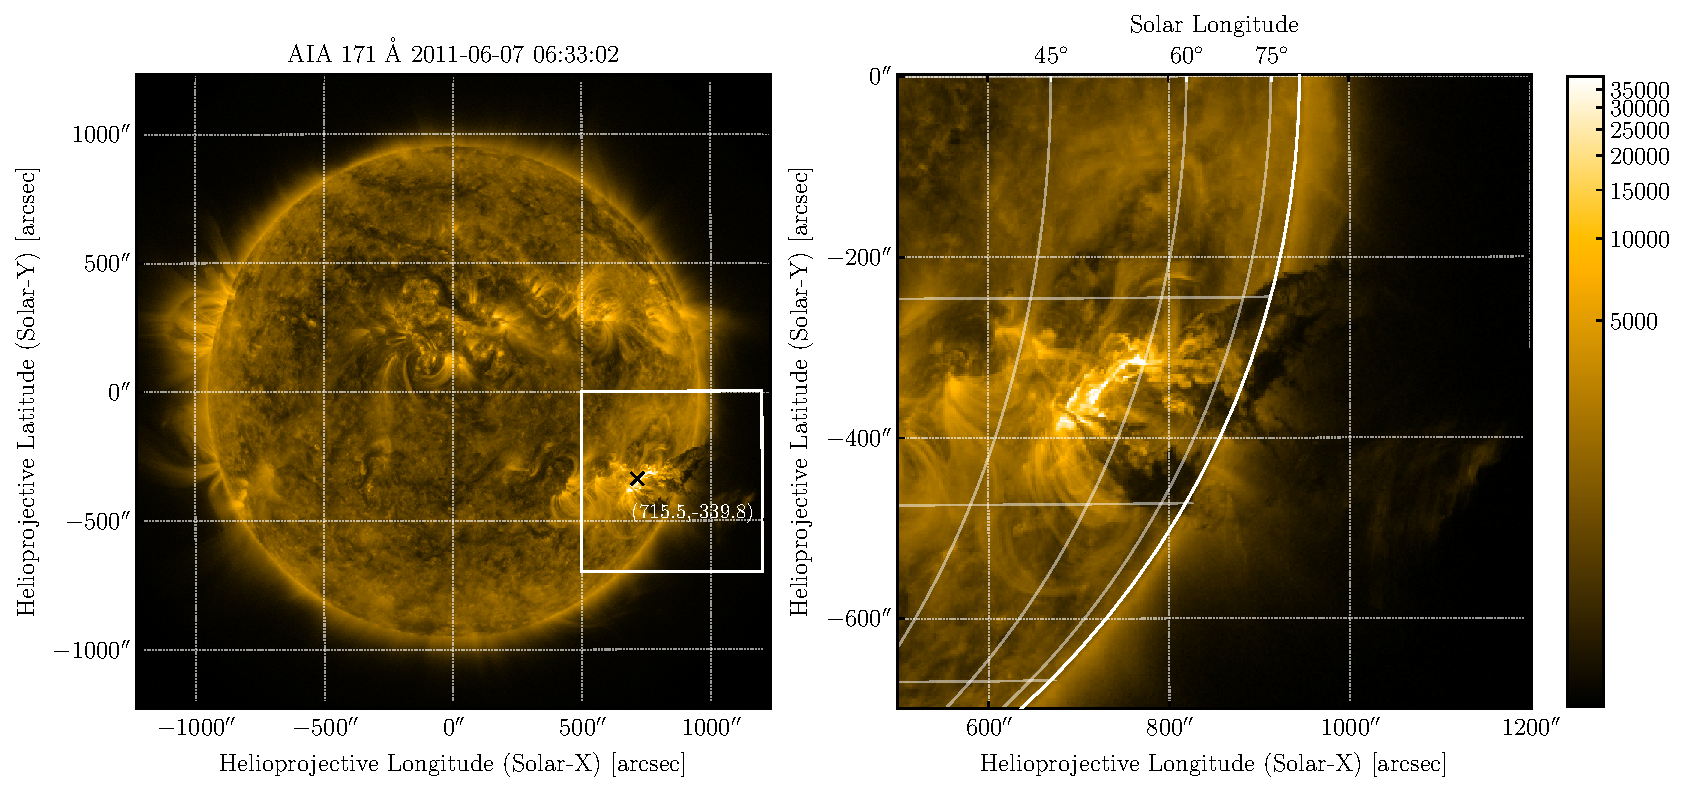
\includegraphics[width=0.55\textwidth]{figures/map_example.pdf}
    \caption{An example of a solar extreme ultraviolet \Map from the Atmospheric Imaging Assembly (AIA) aboard the Solar Dynamics Observatory (SDO).}
    \label{fig:map_example}
\end{figure}

\Map currently supports the data sources listed in Table \ref{tab:instruments} as well as the Helioviewer JPEG2000 image files of for each of these data sources. Due to its flexible data structure, it is easy to add additional instruments and data sources to the \Map object.
